\documentclass[12pt]{article}

% set margins and spacing
\addtolength{\textwidth}{1.3in}
\addtolength{\oddsidemargin}{-.65in} %left margin
\addtolength{\evensidemargin}{-.65in}
\setlength{\textheight}{9in}
\setlength{\topmargin}{-.5in}
\setlength{\headheight}{0.0in}
\setlength{\footskip}{.375in}
\renewcommand{\baselinestretch}{1.0}
\linespread{1.0}

% load miscellaneous packages
\usepackage{csquotes}
\usepackage[american]{babel}
\usepackage[usenames,dvipsnames]{color}
\usepackage{graphicx,amsbsy,amssymb, amsmath, amsthm, MnSymbol,bbding,times, verbatim,bm,pifont,pdfsync,setspace,natbib}

% enable hyperlinks and table of contents
\usepackage[pdftex,
bookmarks=true,
bookmarksnumbered=false,
pdfview=fitH,
bookmarksopen=true,hyperfootnotes=false]{hyperref}

% define environments
\newtheorem{definition}{Definition}
\newtheorem{fact}{Fact}
\newtheorem{result}{Result}
\newtheorem{proposition}{Proposition}



\begin{document}
\title{Taxes and Tariffs}
\author{Kathryn Sarrge\thanks{Syracuse University, Economics Department. Email: kbuzard@syr.edu.} \and Dylan Thomas\thanks{abc} \and Umar Bilgrammi\thanks{abc}}
\date{\vskip-.1in \today}
\maketitle

\vskip.3in
\begin{center} {\bf Abstract} \end{center}

\begin{quote}
{\small Insert abstract text here: 75-200 words, very high-level summary of your project.}
\end{quote}

\bigskip
\section{Introduction} \label{sec:introduction}

Answer the questions
\begin{enumerate}
    \item \textbf{Why should the reader care? / Why is the topic important?} (required)
    \item Why did you choose this topic? (optional)
    \item \textbf{What question will you answer? How will you do it?} (required)
        \begin{enumerate}
            \item If your theory/hypothesis fit in one paragraph, include it here. If it is longer, make it a separate section after the lit review. EITHER OPTION IS FINE as long as the length is sufficient/appropriate for your project.
        \end{enumerate}
    \item \textbf{What did you find?} (required)
    \item \textbf{Give a "road map" of the paper. Where will the reader find the various parts of your work?} (required)
\end{enumerate}

\section{Literature Review} \label{sec:literature}

Discuss at least five papers that are closely related to your results (more is better). Explain how they're related. Did you find something similar, or different? Did you look at a different context? Different time period? Different level of detail?

\section{Theoretical Analysis}
\label{sec:theory}
Optional--may include in intro if it's short.


\section{Data}
\label{sec:data}

Our data consists of two time series datasets that are both provided by the World Integrated Trade Solution website. Both of these datasets provide information in terms of percent of revenue from 1988 to 2022, giving us a 34 years of data to look at from both datasets. The datasets give observations on developing countries and how they have experienced different levels of tariffs on international trade or taxes on goods and services based on the overall revenue of the country. Additionally, both of these datasets have 194 countries, allowing us to combine these datasets easier. The data sets can be acquired through from the \href{https://wits.worldbank.org/CountryProfile/en/Country/BY-COUNTRY/StartYear/1988/EndYear/2022/Indicator/GC-TAX-GSRV-VA-ZS}{World Integrated Trade Solution}  website. To get the data, we altered the indicator on the website allowing us to get our two different data sets. Specifically, we used the indicators Taxes on Goods and Services (percent of revenue) and Taxes on international trade (percent of revenue). We downloaded these datasets by clicking the download button on the table view tab located on the right hand side above the data. In terms of differentiating our two datasets, one focuses on International tax data from developing countries given as a percent of revenue and the other is about international trade data from developing countries given as a percent of revenue. Both these datasets provide data on a per year basis. Since these datasets only have one variable plus one variable per statistical question, these will be the two variables we examine when conducting our analysis. As our data originated in excel, we had to export the data into Stata to clean and transform our data. Firstly we converted our datasets from wide to long individually in Stata and renamed our variables, allowing for easier use of the data and proper formatting. We then combined these datasets using the merge command, creating our \href{https://github.com/ecn310/course-project-taxes-tariffs/blob/main/merged.dta}{merge.dta} file which is our data in it's correct format. In terms of cleaning our data, most data points contained actual observations, therefore we did not need to remove any data point from our dataset. All file documentation will occur in an issue named \href{https://github.com/ecn310/course-project-taxes-tariffs/issues/6}{Data Use Log} in our repository. We also have saved .do files of the data after converting each of them from wide to long name \href{https://github.com/ecn310/course-project-taxes-tariffs/commit/cc891cfec48f11c6a0b9c1aeb2ae980147232ff4}{vat data} and \href{https://github.com/ecn310/course-project-taxes-tariffs/commit/cc891cfec48f11c6a0b9c1aeb2ae980147232ff4}{international data}. Additionally, you the links to access our data are named \href{https://wits.worldbank.org/CountryProfile/en/Country/BY-COUNTRY/StartYear/1988/EndYear/2022/Indicator/GC-TAX-INTT-RV-ZS}{International tax link} and \href{https://wits.worldbank.org/CountryProfile/en/country/by-country/startyear/LTST/endyear/LTST/indicator/GC-TAX-GSRV-RV-ZS}{Taxes on goods and services link}. Our raw data is stored as excel spreadsheets and are named \href{https://github.com/ecn310/course-project-taxes-tariffs/blob/main/VATdatasheet.xlsx}{VATdatasheet.xlsx} and \href{https://github.com/ecn310/course-project-taxes-tariffs/blob/main/internationaltaxdatasheet.xlsx}{internationaltaxdatasheet.xlsx}

\subsection{Survey data}

\section{Results}
\label{sec:result}

We have conducted three separate analysis on our final data, all done in Stata. The first analysis we conducted 

\begin{figure}
    \centering
    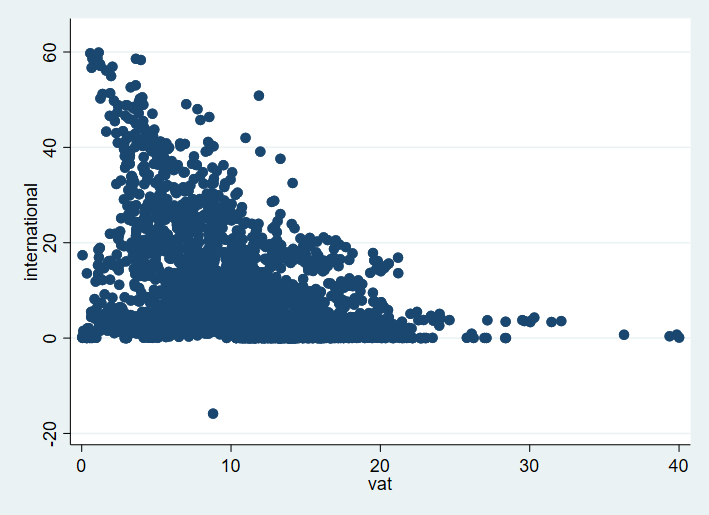
\includegraphics[width=0.5\linewidth]{mergedscatter.png}
    \caption{Merged Data Scatter Plot}
    \label{fig:enter-label}
\end{figure}

\begin{figure}
    \centering
    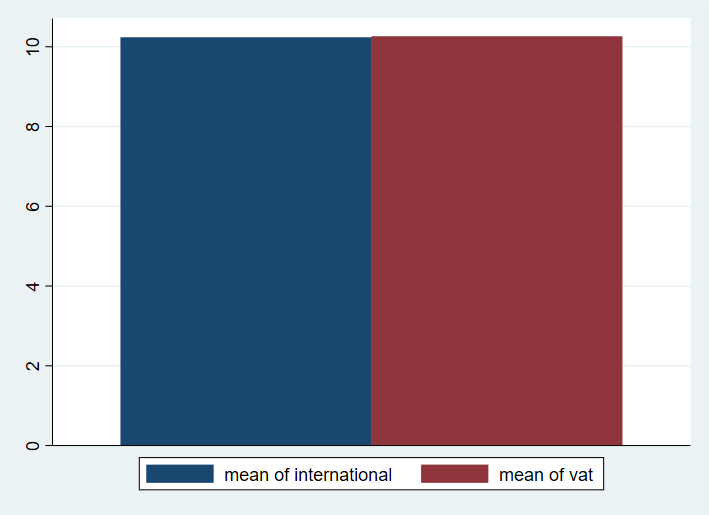
\includegraphics[width=0.5\linewidth]{mergedbar.png}
    \caption{Merged Data Mean Bar Graph}
    \label{fig:enter-label}
\end{figure}

\begin{figure}
    \centering
    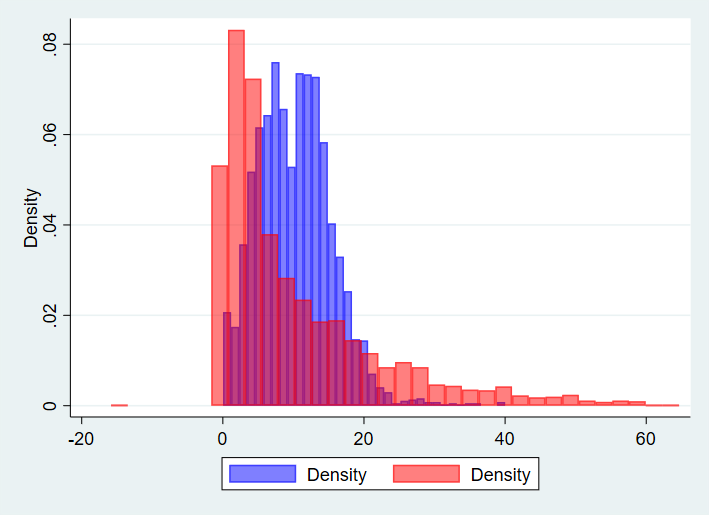
\includegraphics[width=0.5\linewidth]{.github/mergedhistogram.png}
    \caption{Merged Data Histogram}
    \label{fig:enter-label}
\end{figure}




Explain what analyses you did, provide evidence (like in the descriptive stats exercise, but refined and clear) and then explain what your results mean.




\section{Discussion}
\label{sec:discussion}

Optional. This is where you would discuss any of the following
\begin{itemize}
    \item caveats (are there problems with the data that there are no obvious ways to resolve? if so, how might this impact
    \item future work / next steps
    \item implications of the results: that is, how your findings -- if they were causally identified -- might inform policymaking, etc.
\end{itemize}

\section{Conclusion}
\label{sec:conclusion}

Re-state (in different words) what you did and what you learned. If your discussion (Section 6) would be short, you can just have a Conclusion section that includes your discussion (that is, leave out a separate Discussion section).

\newpage
\section*{Bibliography}
\singlespacing
\setlength\bibsep{0pt}

You can either explicitly include your list of references, or you can learn to use BibTex so that it includes the references automatically.

Either way, this list should include ONLY the papers (reports, book chatpers, etc.) that you actually cite in the text (no extra).

At the same time EVERYTHING you cite in the main text must have an entry here (no references in text that don't have something here).

You can choose which citation style to follow. Whichever you choose, you must follow it consistently.

\newpage
\section*{Data Appendix} \label{sec:appendixa}
\addcontentsline{toc}{section}{Appendix A}

You should at least direct your reader to your replication package. You might put key elements of your replication package in this section as well.

\end{document}